\documentclass{standalone}
\usepackage{forsyde-pc}
\usepackage{forsyde-math}
\begin{document}

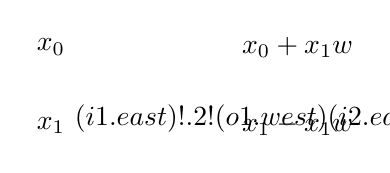
\begin{tikzpicture}[node distance=1cm, auto,]
  \node[anchor=east] (i1) at (0,1) {$x_0$};
  \node[anchor=east] (i2) at (0,0) {$x_1$};
  \node[anchor=west] (o1) at (2,1) {$x_0 + x_1w$};
  \node[anchor=west] (o2) at (2,0) {$x_1 - x_1w$};
  \signal[] (i1) - (o1); \signal[] (i2) - (o2);
  \signal[] ($(i1.east)!.2!(o1.west)$) - ($(i2.east)!.8!(o2.west)$);
  \signal[] ($(i2.east)!.2!(o2.west)$) - ($(i1.east)!.8!(o1.west)$);
\end{tikzpicture}

\end{document}

%%% Local Variables:
%%% mode: latex
%%% TeX-master: t
%%% End:
